\documentclass[12pt]{scrbook}

\usepackage{mdframed}
\usepackage{anyfontsize}
\usepackage{adjustbox}
\usepackage{graphicx}
\usepackage{latexsym}
\usepackage{amssymb}
\usepackage{theorem}
\usepackage{makeidx}

\usepackage{listings}
\usepackage{color}
\lstloadlanguages{Python}
\definecolor{dkgreen}{rgb}{0,0.6,0}
\definecolor{gray}{rgb}{0.5,0.5,0.5}
\definecolor{mauve}{rgb}{0.58,0,0.82}

\lstset{frame=tb,
  language=Python,
  aboveskip=3mm,
  belowskip=3mm,
  showstringspaces=false,
  columns=flexible,
  basicstyle={\small\ttfamily},
  numbers=left,
  numberstyle=\tiny\color{gray},
  keywordstyle=\color{blue},
  commentstyle=\color{dkgreen},
  stringstyle=\color{mauve},
  breaklines=true,
  breakatwhitespace=true,
  tabsize=3
}

\newcommand{\sbsmedia}{{\Large\sffamily Story Byte Studios}}

\mdfdefinestyle{l3style}{%
leftmargin=0pt,
backgroundcolor=black,
fontcolor=white,
linewidth=0pt,
innertopmargin=20pt,
innerbottommargin=20pt,
innerleftmargin=20pt,
font={\fontsize{50}{40}\selectfont}
}

%% ENVIRONMENTS =====================

\theoremstyle{plain}
\newtheorem{Exe}{Exercise} 

\theorembodyfont{\rmfamily}
\theoremheaderfont{\scshape}
\newtheorem{Exp}{Expert Knowledge}
\newtheorem{Gmd}{Game Design}

\newcommand{\expend}{\hfill$\blacktriangleleft$}

%% INDEX =============================

%% A


%% B
\newcommand{\boolean}{Boolean\index{Boolean}} 
\newcommand{\breakloop}{\texttt{break}\index{\texttt{break}}}

%% E
\newcommand{\event}{event\index{event}}

%% F
\newcommand{\flag}{flag\index{flag}}
\newcommand{\forloop}{\texttt{for}\index{\texttt{for} (loop)}} 
\newcommand{\function}{function\index{function}}


%% G
\newcommand{\gamemechanic}{game mechanic\index{game mechanic}} 

%% I
\newcommand{\integer}{Integer\index{Integer}} 
\newcommand{\infiniteloop}{infinite loop\index{infinite loop}} 



%% L
\newcommand{\pythonloop}{loop\index{loop}} 

%% S
\newcommand{\strvar}{String\index{String}} 

%% V
\newcommand{\victorycondition}{victory condition\index{victory condition}} 

%% W
\newcommand{\whileloop}{\texttt{while}\index{\texttt{while} (loop)}} 
\makeindex

%% REFERENCES ======================

\newcommand{\exeref}[1]{Exercise \ref{#1}}
\newcommand{\figref}[1]{Figure \ref{#1}}


%% DOCUMENT =========================

\begin{document}

\pagestyle{empty}


\vspace{5em}

\begin{flushleft}
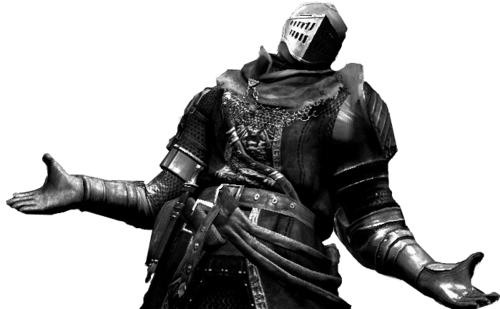
\includegraphics[scale=.88]{images/darkknight.png}
\end{flushleft}

%\vspace{-2.5em}

{\noindent\Large\emph{Programming}}\vspace{-0.3em}

\begin{mdframed}[style=l3style]
Adventure Games \par
\hspace{-.2cm}in Python
\end{mdframed}

\vspace{1em}


\begin{adjustbox}{minipage=.3\textwidth,right}
\Large\em
Geert-Jan Kruijff
\end{adjustbox}

\vfill

\sbsmedia

\tableofcontents 

% Introduction to the book
% Started: Wed 3 Oct 2018 


\chapter{Introduction} 

\section{Creating Adventures} 




\section{For Whom Is This Book?}


\section{Getting Things Set Up} 




\subsection{Mac} 

\subsection{Windows} 


\section{Conventions Used in This Book}


\section{Code Examples}

\section{Using Code Examples}

\section{Contacting the Author}



% Part 1 -- Getting started 

\part{Getting Started} 
\chapter*{Introduction to Part 1} 

Let's get started! In this part we are going to cover quite some ground ... We start right away with building a simple, text-based adventure. Hello adventure world! We then continue with learning how we can let the player make decisions (i.e. actually play the game!), and how we can keep track of what all is happening. Towards the end of this first part, we build things out to a fully-fledged game engine that can run "any" kind of text adventure. 

Specifically, you will learn: 
\begin{itemize}
\item How to use \textit{Atom}, \texttt{git}, to edit, run, and version your programs
\item How to let your program show something in a Terminal (\texttt{print}), and get some input from your user (\texttt{input})  
\item How to implement basic control structures in Python, for decisions (\texttt{if..then..else}) and loops (\texttt{while...} loops, and \texttt{for} enumerations) 
\item How to define functions, classes, and modules in Python (and what these things are! and why they are useful!)  
\item How to store your adventures as files, using a structured file format (\textit{JSON})
\item How to save games, and load them, and how to load game resources 
\end{itemize}


 
\chapter{Hello Adventure World} 

\section{Introduction}

A program is basically a set of instructions what to do. There are different programming languages we can write such instructions in -- Python is one of them. Other languages are for example Java, C, C++, Swift -- by now (October 2018) probably close to 300 different programming languages exist! But, we will just focus on Python for the moment. 

Python is actually more than "just" a language. It is also a program that can interpret your program and then translate it into instructions for your computer to execute. Let us see that in action right away. 

Open a terminal, type in \textbf{\texttt{idle3 \&}} after the \$-prompt, and press return: 

\begin{itemize}
\item[\$] \textbf{\texttt{idle3 \&}}
\end{itemize}

Up pops a little window, like the one below.  
 
\begin{figure}[h]
\centerline{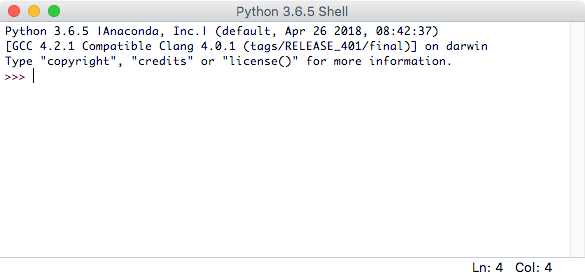
\includegraphics[scale=.70]{images/p1ch1-idle3.png}}
\caption{The Python IDLE3 interactive editor}
\end{figure}

This is the \texttt{idle3} window. It is an interactive editor for Python. Everything you type in is immediately interpreted and executed -- so you can see right away what it does! 
Let's see this at work. After the "$>>>$" prompt in the editor, type in the following: 

\begin{itemize}
\item[$>>>$] \textbf{\texttt{print("Hello Adventure World!")}}
\end{itemize}

And there you go! Right below your command, \texttt{idle3} shows the text "Hello Adventure World!" -- you have written \emph{and} executed (or "ran") your first line of Python code!

\begin{itemize}
\item[$>>>$] \texttt{print("Hello Adventure World!")}\\
	\textbf{\texttt{Hello Adventure World!}}
\end{itemize}

Feel free to try out more -- how do you imagine your adventure would start? Where does the player start, what does he -- or she -- see, smell, feel? 

\begin{itemize}
\item[$>>>$] \textbf{\texttt{print("You are in a dark, spooky house, hidden deep in the forest. \\ 
		   There is only one door to the outside, and it is locked. You hear \\ 
		   strange, creaky sounds. What do you do?")}}
\end{itemize}
   
Sometimes such a long piece of text looks kind of awkward. If you want to break things up a little, you can insert a \texttt{$\backslash$n} or "new line" in your text. For example, if we want to have each sentence start at a new line, we can achieve that as follows: 

\begin{itemize}
\item[$>>>$] \textbf{\texttt{print("You are in a dark, spooky house, hidden deep in the forest.$\backslash$n\\ 
		   There is only one door to the outside, and it is locked.$\backslash$n \\
		   You hear strange, creaky sounds.$\backslash$n\\
		   What do you do?$\backslash$n")}}
\end{itemize}
   

\section{Your First Real Program}    
   
The \texttt{idle} interactive editor is useful to try a couple of things out, and see what they do. However, you can only do things line by line, and have to retype everything if you want to try again! In this section move to using \textit{Atom}, a so-called "interactive development environment" or IDE. We will use editor to type in programs, run them, and store versions in \texttt{git}.

Start up \textit{Atom}, and click on the "Welcome Guide" tab. The window will look something like what you see below. 

\begin{figure}[h]
\centerline{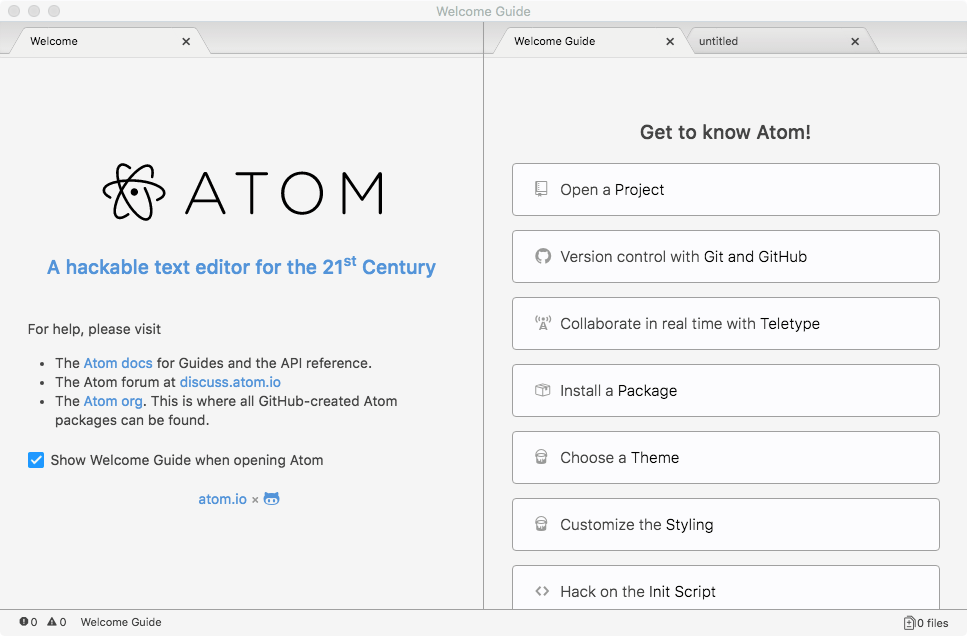
\includegraphics[scale=.2]{images/p1ch1-atomwelcome.png}}
\caption{Atom with the Welcome Guide selected}
\end{figure}

We start by creating a new project. Click on the "Open a Project" tab, and then the "Open a Project" button. A file browser pops up. Go to the Desktop, create a new folder there called "pythonadventures" and then click the "Open" button. Atom now opens a \textit{Project} pane on the right hand side. 

\begin{figure}[h]
\centerline{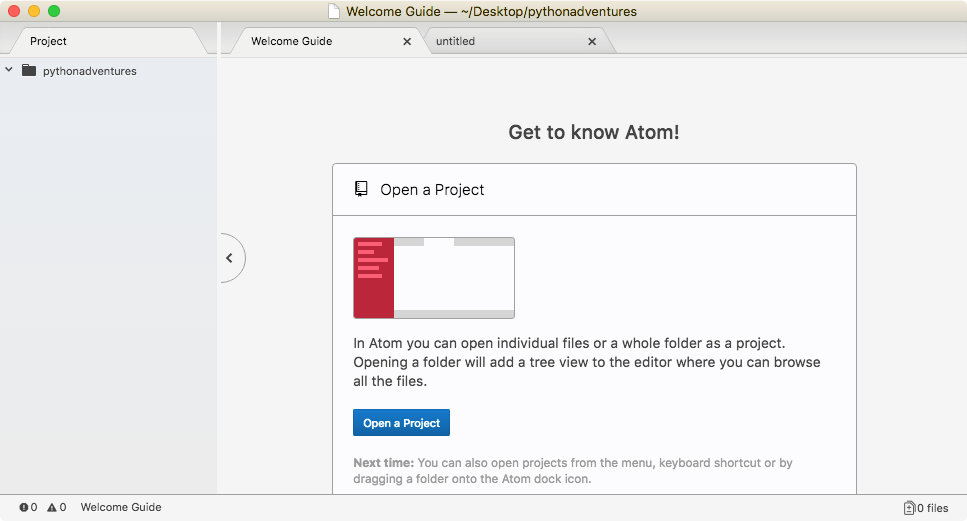
\includegraphics[scale=.20]{images/p1ch1-projectbrowser.png}}
\caption{Atom with the Project pane and browser}
\end{figure}

Next, we want to add a \texttt{git} "archive" or \emph{repository} to our project. There are two ways in which we can do that. One, we can scroll down in the Welcome Guide tab, till you see the "Version control with Git and GitHub" tab. There are two buttons there, "Open the Git panel" and "Open the GitHub panel." If you want you can click on the "Open the Git panel" -- or wait and see how we can get to that panel more quickly. If you hover with your mouse on the middle of the right side of the window, a half moon button pops up with a "$<$" inside. Click on that button to directly get to the Git panel! 

Now, because we already set up our project, the Git panel has a button that suggests we create a repository directly in our project directory. As that is exactly what we want, press the button, and then click "+Init" in the window that pops up to initialize the repository ("repo") in the directory as shown.  

Finally, select the "untitled" tab, so that we can get coding! Atom now looks like below, (and you may have noticed already that the Project browser has been updated with a ".git" folder -- our repository). 

\begin{figure}[h]
\centerline{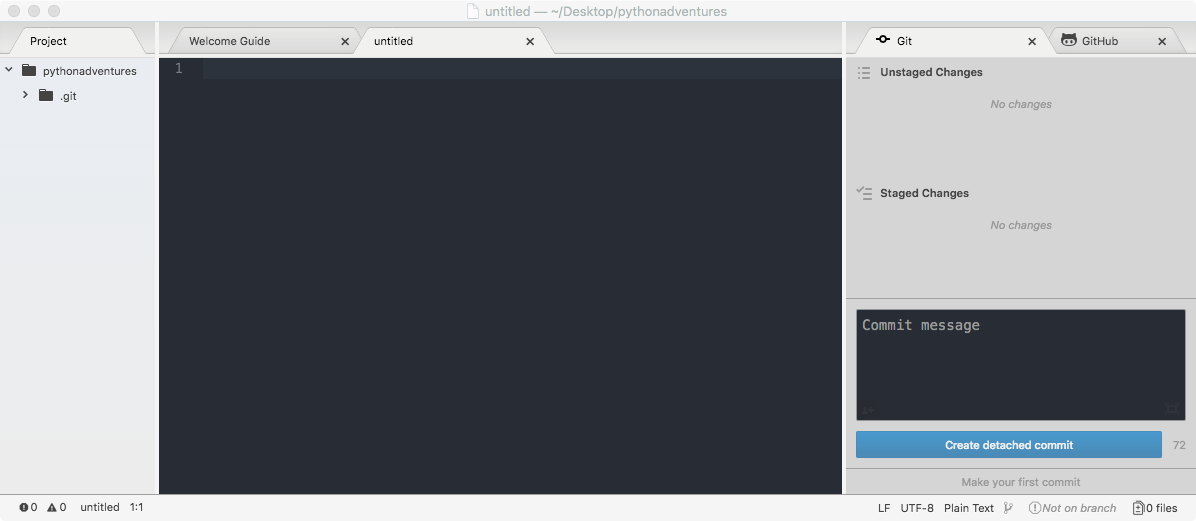
\includegraphics[scale=.20]{images/p1ch1-gituntitledprojectbrowser.png}}
\caption{Atom with the Project pane, the Git pane, and the code editor}
\end{figure} 

Type in the following lines of code in the editor. The line numbers below reflect those you see in the editor. 

\pagebreak

\begin{lstlisting}
1. print("You are in a dark, spooky house, all alone out in the forest.")
print("You are in a dark, spooky house, all alone out in the forest.")
print("There is only one door to the outside, and it is locked.")
print("You hear strange, creaky sounds.")
print("What do you do?")
command = input("> ") 
\end{lstlisting}


Once you have entered the code, and save it in the project directory as \emph{p1ch1-pythonadventure.py}. In the Project panel the file now appears, and \texttt{git} has also spotted that there is something now! Notice that our file is listed under "Unstaged changes." Before \texttt{git} puts something into the repository, you need to "stage" it. Click on "Stage all" to move your file to the "stage." Then, in the \emph{Commit message} you should type a simple and short description of what is new or different in the file(s) you have staged. Right now this is simple: "everything is new!" Next, push the \emph{Commit} button. Because our repository is empty, the button says "Commit detached." Push the button, to make your first commit to the repository. Well done!

\begin{Exp}[The \texttt{git} master, and branches] 
The Commit button now says "Commit to master." The \emph{master} is the main archive. People often visualize the archive as a tree, where the main archive is the "trunk," from which you can also create "branches." A branch initially diverges from the trunk, allowing you to try things out without these experiments ending up in the main archive. This can be handy: If we decide the experiments are no good, we cut the branch and no harm is done to the main archive. If instead we decide that all is great, then we can merge the branch with the trunk to have the main archive reflect all the changes we made.      \expend 
\end{Exp}
 
 
 
Stage all, 
write something in the commit window, 
Push button to Commit detached
(Later this goes directly to Master) 




   
   
    	% part 1, chapter 1: print, input(), git  
\chapter{Making Decisions} 

\section{Introduction} 

At the end of the previous chapter we saw how we could get the user to type something in, and then advance the story. In this chapter, we explore this further. We start with the user simply pressing \emph{Enter} to advance the story, just like turning a page. Then, we look at \textit{variables}, for example \textit{String} variables that can hold text. We use a variable to pick up what the player just typed in -- remember \texttt{command}? Once we have that, we inspect what the player wants to do (e.g. look around, or go south) and drive the story forward accordingly. For that, you learn more about the \texttt{if..then..else} control structure in Python, and basic String comparison \texttt{==}. By the end of the chapter, we will have a game where the player can roam around various rooms in the house, look around, and find all manner of horrific things ... 

\section{The Story So Far} 

So far, the story is that you are in "a dark, spooky house, all alone out in the forest." Scary thing is, you are inside -- and you cannot get out! Whereas, hearing strange noises, getting out is clearly what you want ... 

 \begin{Gmd}[Victory condition] Most games have a \textit{\victorycondition}: What you need to achieve to win the game. Collect all the little shiny boxes, like in \emph{Fez}, or defeat all the monsters, like in \emph{Dark Souls}, or free the princess in \emph{Super Mario}. (Not all games have apparent victory conditions, for example look at an exploration game like \emph{Dear Esther}.) Key is of course that the player has some idea about what the victory condition might be. In our story, the first few lines already make it clear: Escape! Which then turns into the question, how ....  \expend  
  \end{Gmd} 
  
  Having some idea about what you need to achieve is good, but even better is knowing \emph{how} you can achieve it! This is where \gamemechanic{s} and \event{s} come into play (literally).   
      
  \begin{Gmd}[Game mechanics and events] A \textit{\gamemechanic} defines how the game works. It is a rule we implement in code, determining what a player can do. If the player does "this," then "that" is going to happen. For example, many games use the \emph{A} button on the (Xbox) controller to make your character jump. That is a mechanic. Or, in text adventures, you type in a command -- that is another mechanic. When you are playing a game, you use these mechanics to make things, \textit{\event{s}}, happen. Things may go one way or the other, depending on what you decide to do. Take again \emph{Dark Souls} -- as the monster attacks you, do you press \emph{L1} to raise your shield and block the attack, or do you use your left stick and \emph{O} to roll to the side? Different mechanics, allowing you to take different actions, resulting in different ways in which the game might play out ...   \expend
  \end{Gmd}
  
Let's use that to work out our story a little bit more. The \victorycondition\ is to get out of the house but the only door outside is locked. Let's assume that that means the player needs to find a key. As the game wouldn't be particularly exciting if the key would be laying there right in front of the player's nose, we need some \gamemechanic{s} for the user to go around the house, and look for objects. And that should, of course, lead to some "interesting" events ...  

\begin{figure}[h]
\centerline{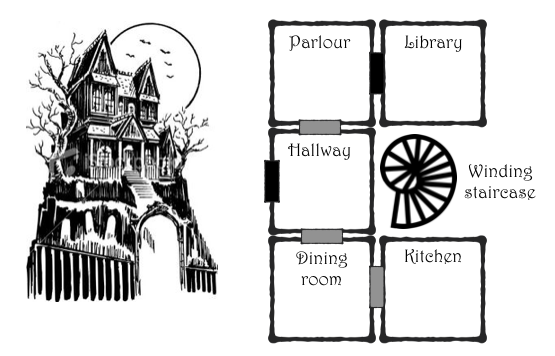
\includegraphics[scale=.70]{images/p1ch2-hauntedhousemap.png}}
\caption{The Haunted House In The Forest}\label{fig:hauntedhousemap}
\end{figure}

\figref{fig:hauntedhousemap} shows the map of the house. The black and grey triangles indicate doors. Grey means the door is open, black means that door is closed. The player needs to find the right key to open a closed door. The player can find the key to the \emph{Library} in the \emph{Parlour}. The key to the door outside is in a handbag in the \emph{Kitchen}. 

Now, this would not be a scary story if there would not be any monsters around ... So let's place a Ghoul in the kitchen, to guard the Key To Outside. This is going to be our \emph{Boss Fight}! 

We should not allow the user to simply waltz into the kitchen, completely ignore the Ghoul, and just grab the key. No -- if the player does that, "You Died!" Instead the player needs to find a weapon to defeat the Ghoul. The Library is a good place for that. We can put a sword above the mantelpiece. For good measure we also put a Ghost in the Library. The Ghost floats in front of the sword. 

Those are our key objects: the key to get into the Library (found in the Parlour), the sword to kill the Ghoul (found in the Library), and the key to get out of the house . The player can find that final key in a handbag in the Kitchen. To spice things up, we can let the Ghoul carry the handbag around its neck.  

We now have our locations, our objects, a monster -- what we need now still is define what the player can do. 

We have objects, so a player should be able to \textbf{take} an object -- "take sword" or "pick up key." 

We are not going to place these objects in plain sight, as that would be too easy. The player should \textbf{search} -- "search room" or "look in handbag." 

Naturally, the player needs to be able to get around the house. We can do that "old school"-style using \textbf{go} with a compass direction -- "go north", "go south." From the Hallway you can go North to the Parlour, or South to the Dining Room, etcetera. 

Finally, as we have monsters, the player needs to be able to \textbf{attack} a monster -- or \textbf{retreat} if the monster is too scary! 

Okay, there we go. All we need now is the story ... and the code. 

\section{Getting The Story Going} 

Let us have a look again at the code we have so far. 

\begin{lstlisting}
print("You are in a dark, spooky house, all alone out in the forest.")
print("There is only one door to the outside, and it is locked.")
print("You hear strange, creaky sounds.")
command = input("> ")
print("Boo!")
\end{lstlisting}

As our story is going to continue well beyond the cheap jump scare in line 5, we can delete the "Boo!" Instead, we should take stock of the situation. What do we know? Well, we know that the player does \emph{not} have the main key, nor the key to the library, nor the sword -- nor the handbag for that matter. All of that is key to achieving the victory condition: 

\begin{enumerate}
\item Search the Parlour to find the key to the Library
\item In the library, attack the Ghost, then take the sword
\item In the kitchen, use the sword to attack the Ghoul
\item After the Ghoul has been defeated, take the handbag
\item Search the handbag, find the main key
\end{enumerate} 

Once the player has the main key, he should go to the Hallway, and escape the haunted house. Game over, "You Win!"

This means we need to track what the player already has. We can use variables for that. A variable is essentially a "container" you can put a value in (assign a value to). For example, look at line 4 again: 

\begin{verbatim}
command = input("> ")
\end{verbatim}      

We introduce here a variable \texttt{command}, to which we assign a value we get from the function \texttt{input} -- i.e. command stores what the user has just typed in. In Python, there are various types of variables. The \texttt{command} variable is a variable of type \textit{\strvar}. A \strvar\ stores text. If the user types in \textit{go south} and presses enter, then the \emph{value} of \texttt{command} becomes 'go south'. 

\begin{Exe} 
Try this out in \texttt{idle}. Type line 4 in \texttt{idle}, and then type in a command. After you have pressed enter, type in \texttt{command} (the variable name), and press enter again. \texttt{idle} shows the value assigned to that variable.  \expend
\end{Exe}

There are also various other types of variables. Two types you will frequently encounter are \textit{\integer} variables, and \textit{\boolean} variables. An \integer\ variable stores (whole) numbers. 

 \begin{Exe} 
Try this out in \texttt{idle}. Type in \texttt{score = 0}. You have zero points! To check that, type in \texttt{score} (and press enter), and you will see -- 0. If you want a higher score than that, simply add that to the variable, like so: \texttt{score = score + 100}. This means, "take the current score, add 100, and store the resulting number again in score." Now add another 10 points, and check what value is assigned to \texttt{score}. \expend
\end{Exe}

\begin{Exp}[Integer addition short cut] 
If all you want to do is add a number to the current value of an \integer\ variable, and assign the result again to that variable, (like we did above), then Python has a shortcut for that. Instead of \texttt{score = score + 100} you can also use the short-cut \texttt{score += 100}. \expend
\end{Exp} 
 
A \boolean\ variable is a variable that is either \texttt{True} or \texttt{False}. We can use such variables to track whether the player has certain items. Does the player have the sword? The main key? At the beginning -- none of that, so we set all those variables to \texttt{False}. 

We often call such \boolean\ variables "\flag{s}"  A flag variable is a variable you define to have one value until some condition is true, in which case you change the variable's value. For example, \texttt{hasSword = False} until the player has taken the sword in the Library -- then it becomes \texttt{True}.  It is a variable you can use to control the flow of a function or statement, allowing you to check for certain conditions. So, only once it is the case that \texttt{hasSword = True}, the player can attack the Ghoul and stand a chance to survive that encounter. 

Type in the code below, before the first \texttt{print} line. Something new: Lines 1 and 6 start with \texttt{\#}. This indicates a comment; Python happily ignores those lines. Note that you do not need to retype all the print statements; the full code listing is included for illustration. 

\begin{lstlisting}
# Initialize flags 
hasMainKey = False 
hasHandbag = False
hasSword = False 
hasLibraryKey = False 
# The story begins -- the Hallway
print("You are in a dark, spooky house, all alone out in the forest.")
print("There is only one door to the outside, and it is locked.")
print("You hear strange, creaky sounds.")
command = input("> ")
\end{lstlisting}

What is the first thing that the player might do in such a situation, other than scream "lemme out!?!"? Well, either of two things. Either the player indeed says "help," or something like "look around." If the player says "help", we can help him (or her) out by saying some soothing words, and briefly explain what actions can be performed. Type in the code below. After the code we explain what this new \texttt{if..} construction means.   

\begin{lstlisting}[firstnumber=last]
if (command == "help"):
    print("Don't be scared. You can do a couple of things:")
    print("- 'go' in a compass direction, e.g. 'go south' ")
    print("- 'search' to 'search room', or look into an object")
    print("- 'attack' to attack a monster")
    print("- 'take' an object, e.g. 'take key' ")
\end{lstlisting}

The \texttt{if} statement in line 11 is a check. If the player typed in \textit{help}, then do whatever comes after the \texttt{:} -- in this case, several print statements. For Python it is very important that the block of code that should be executed, is properly \textit{indented}. As you can see, the \texttt{print} statements do not begin at the same position as the \texttt{if} position, but a little further. Atom does this automatically. 

Another thing you may notice is that we use a double "==" and not a single "=" to make a check. This is important, and makes all the difference. A single "=" \emph{assigns} a value to a variable -- a statement \texttt{score = 10} assigns the value 10 to the variable \texttt{score}. A double "==" compares the value of the variable, to the value provided. So, \texttt{score == 10} is a check whether the score is 10 (or not) -- or, as in line 11, we check whether the player's command was "help."   

\begin{Exp}[Single or double quotes?] 
Finally, once we are talking about things you may be noticing: When you used \texttt{idle} to check the value of a \strvar\ variable, the value was returned with single quotes, e.g. \texttt{'help'}. But now, line 11 is using double quotes -- \texttt{"help"}! Why, what is the difference? Simple answer: There is no difference. You can use double quotes or single quotes, and to Python it is all the same. In general, we use double quotes here, and in lines 12 through 16 you also see we are using single quotes inside double quotes ... not a problem. \expend 
\end{Exp}

The following code provides the player with more details about the Hallway, should he be looking around. Looking at the map in \figref{fig:hauntedhousemap} (on p.\pageref{fig:hauntedhousemap}) again, we see that the player has several possibilities. 

\begin{lstlisting}[firstnumber=last]
 if (command == "look around"):
    print("You find yourself in the hallway.")
    print("To the east is a winding staircase, on the verge of collapse.")
    print("To the west is the door to the outside.")
    print("You can go north, and south.")
\end{lstlisting}

Before we let the player go to the Parlour, let's handle the case where somebody is really scared and desperately wants to get out of this house as fast as possible. What if the player says \texttt{go west}? Well, if the player has the main key -- fine, go ahead, you win. But if not ... So what we need to do, after checking whether the command is \texttt{go west}, is what the status of our \texttt{hasMainKey} flag is. No key? No exit. 

\begin{lstlisting}[firstnumber=last]
if (command == "go west"):
    if (hasMainKey == True) :
        print("You have escaped the house! You can breathe easy now.")
    else:
        print("The door is locked. You need a key...")
\end{lstlisting}

Line 23 checks whether the player has the key. If that is the case (\texttt{hasMainKey == True}), then the player wins. If that is \emph{not} the case, then we get to the \emph{else} statement in line 25. Note that this other case means \texttt{hasMainKey} is \texttt{False}, as a \boolean\ can only have one of these two values. The player is informed that he cannot go ("oh nooooo.....") but he does get a little hint: go look for the key ... 

\begin{Exe}
Run the program in the terminal. Type in a command. What happens, after you have typed in the command? \expend
\end{Exe}

(In case you read this already without doing the exercise first -- no cheats or shortcuts!) Indeed. After you have typed in a command (help, look around, go west), the program ends. That's not much of an adventure of course, so we should change that. Add another statement \texttt{command = input("> ")} at the end of the long \texttt{print} blocks for "help" and "look around", and at the end of the "else" block (after line 26). Make sure to use the right indentation!  
      
\begin{Exe}\label{exe:fixedorder}
Run the program in the terminal. Type "help." After that, try "look around." Does that work? Now try "go west." What happens if you \emph{now} type in "look around"? Can you explain why?\footnote{The answer: We go step-by-step through the program, and in this program you cannot go back. So once you are passed "look around" the only next step you can take is "go west" as the program no longer checks for "help." Not great, indeed, but it's a start. Later on we will see how to do better.} \expend
\end{Exe}

It's time to get the player moving around. First, we go north, to the Parlour. There the player can find the key to the Library, and once we are in the Library, there is a Ghost to deal with before the player can then take the sword ... 

\begin{lstlisting}[firstnumber=last]
if (command == "go north"):
    print("You go through the door, into the Parlour.")
    print("Heavy curtains cover most of the windows. ")
    print("It smells dusty here.")
    print("There is a door to the west, which appears locked.")
    command = input("> ")
    if (command == "look around" or command == "search room"):
        print("In the faint light, you see several chairs, and a coffee table.")
        print("A key is laying on the coffee table.")
        command = input("> ")
    if (command == "take key"):
        hasLibraryKey = True
        print("You found the key to the library!")
        command = input("> ")
\end{lstlisting}
 
Once you have typed in the code above, let's have a closer look. 

First of all, notice the \texttt{or} in line 33. This means: if the player typed in \emph{either} "look around" \emph{or} "search room", execute the block of code after that. So we offer the player a little bit of flexibility here in how he can phrase what he wants to do. 

\begin{Exe}
If you like, go back and change the code in line 17, to match line 33. \expend 
\end{Exe}

Another thing is that we are starting to change our flags. Assuming the player has seen there is a key, and then decided to "take key" we can now set the flag \texttt{hasLibraryKey} to \texttt{True}. 

Alright, so now the player has the key to the library. If the player now says, "go west" -- no problem. Or, if the player has not looked around so far, and thus does not know there is a key to pick up, then "go west" should not take him into the Library. Just like we saw in line 23, we can check our flags, and handle that too. 

Or so it seems ... but first things first. After the block for taking the key, add the following. Make sure that the indentation is at the same level as the \texttt{if}-statements for looking around, and taking the key. 

\begin{lstlisting}[firstnumber=last]
if (command == "go west"):
        if (hasLibraryKey == False):
            print("The door to the library is locked.")
            print("You need the key to the library to open the door.")
        else:
            print("You unlock the door, and enter the Library")
\end{lstlisting}

\begin{Exe}
Do you already see the problem that we are running into? See also \exeref{exe:fixedorder}. \expend
\end{Exe}

Everything is fine as long as the player takes the steps exactly in the order as we programmed them. Look around, take stuff, go somewhere. But, oooh, what if the player does things in another order? The program is going to be messy -- "spaghetti code" as that's sometimes called. If we handle everything in a very strict, linear fashion ("on rails") then we need to take care of every possible order in which the player might be doing something. Suffice to say that that's not a good way to do it. 

So why did we do it that way then in the first place? Well, to show you what it is like. Understand the problem, and then in the next chapter, we discuss how to properly solve it!

\begin{Exp}[Refactoring] 
It often happens that you start programming, and as you go along, you find out that your solution is not quite what it should be. Even though there are local improvements you can still make, you probably realize that ultimately this particular implementation is a dead-end. And that is fine! You have learnt an important lesson -- how \emph{not} to do. Now what you can do is take the pieces of code that you are happy with, and put them together in a different, better way. We call that \emph{refactoring your code}. Remove the spaghetti and the bad ideas, take what is good, then build a new and better solution. \expend    
\end{Exp} 

Still. Although we know now that this is not the way to go, we can still go and extend our code a little bit. There is still a Library to explore, and more importantly, there is a Ghost to scare away. 

\begin{lstlisting}[firstnumber=41]
    if (command == "go west"):
        if (hasLibraryKey == False):
            print("The door to the library is locked.")
            print("You need the key to the library to open the door.")
        else:
            print("You unlock the door, and enter the Library.")
            print("You immediately notice the free floating full torso vaporous apparition.")
            print("In other words, there is a ghost.")
            print("It is floating in front of a sword, hanging above the mantelpiece.")
            command = input("> ")
            ghostPresent = True
            if (command == "look around" or "search room"):
                print("What are you doing?! There is a ghost flying around!")
            if (command == "attack" or "attack ghost"):
                print("You slowly walk towards the ghost.")
                print("The ghost appears to be reading a book.")
                print("As you approach, she looks towards you, about to say 'Shh!'")
                print("You respond with a questionable 'Boo?!' ")
                print("The ghost disappears, whispering 'the kitchen, danger...'.")
                ghostPresent = False
\end{lstlisting}

Just for the purpose of this individual scene, we introduce a \emph{local} variable called \texttt{ghostPresent}. It simply tracks whether the ghost is still here, or not. We initialize it in line 51 to \texttt{True} is the ghost is in the Library when we enter. Only once we have chased it away, with a rather feeble "Boo?!" at that, we set it to \texttt{False} (line 60). If the player now tries to take sword, all is fine. If the ghost however is still there, see what happens. 

\begin{lstlisting}[firstnumber=59]
                print("The ghost disappears, whispering 'the kitchen, danger...'.")
                ghostPresent = False
                command = input("> ")
                if (command == "take sword" and ghostPresent == False):
                    print("You reach up to the sword, and take it.")
                    print("Be careful not to cut your fingers, as it is sharp.")
                    hasSword = True
            if (command == "take sword" and ghostPresent == True):
                print("As you try to reach thru the ghost, to reach the sword,")
                print("She turns into a frighteningly old lady, flies through you,"
                print("and covers you in sticky ectoplasmic goo.")
                print("The ghost is still floating around, muttering angrily.")
\end{lstlisting} 

The code listing above repeats a bit of the previous code, to make sure it is clear how to indent the code. The first "take sword" block is \emph{within} the overall "attack" block, whereas the second "take sword" block is indented at the \emph{same} level as "attack" block. In other words, if you immediately go and grab the sword without attack the ghost first, you will get slimed (rather than get the sword). 

One new thing in the code above is the use of the \texttt{and} operator. Whereas \texttt{or} indicates that one of the conditions for the \texttt{if} must be true, the \texttt{and} indicates that they must \emph{all} be true. 

\begin{Exe} 
Look at line 62. Is the second condition \texttt{ghostPresent == False} needed? How about the statement \texttt{ghostPresent == True} in line 66?\footnote{The answer: Look at what the player must have done to arrive at line 62. He must have attacked the ghost first. That means that there is no need to check, as we know that the ghost is gone. Something similar holds for line 66. We know that the player has not attacked the ghost, so the ghost must still be there. Again, we do not need to check for the condition, as there is only one possible value for \texttt{ghostPresent} at that point. However, if the code would support the player to perform these actions in any order, then these conditions are of course necessary!}   
\end{Exe}  

That's it. Make sure to stage and commit the code to \texttt{git} (cudos if you have been doing that after each step!), and run the adventure. If you stick to the right order, it is definitely fun to play! But, yes, indeed, there is room for improvement. In the next chapter, we look at bringing in the required flexibility, and we will complete the story.  






   		% part 1, chapter 2: variables and if..then
\chapter{Till The Bitter End} 

				% part 1, chapter 3: while loops 
\printindex

\end{document}


